\documentclass[t, 10pt, aspectratio=1610]{beamer}
 % align text inside frame to t=top, b=bottom, c=center
 % 8pt, 9pt, 10pt, 11pt, 12pt, 14pt, 17pt, 20pt available as text font
 % select your aspect ratio 4:3=43, 16:9=169, 16:10=1610

\usetheme{Juelich}
\usepackage{xparse}

%https://tex.stackexchange.com/questions/184991/a-reusable-newlength-no-stop-break-if-length-already-defined

\makeatletter
\newcommand{\providelength}[1]{%
  \@ifundefined{\expandafter\@gobble\string#1}
   {% if #1 is undefined, do \newlength
    \typeout{\string\providelength: making new length \string#1}%
    \newlength{#1}%
   }
   {% else check whether #1 is actually a length
    \sdaau@checkforlength{#1}%
   }%
}

\newcommand{\sdaau@checkforlength}[1]{%
  % get the first five characters from \meaning#1
  \edef\sdaau@temp{\expandafter\sdaau@getfive\meaning#1TTTTT$}%
  % compare with the string "\skip"
  \ifx\sdaau@temp\sdaau@skipstring
    \typeout{\string\providelength: \string#1 already a length}%
  \else
    \@latex@error
      {\string#1 illegal in \string\providelength}
      {\string#1 is defined, but not with \string\newlength}%
  \fi
}
\def\sdaau@getfive#1#2#3#4#5#6${#1#2#3#4#5}
\edef\sdaau@skipstring{\string\skip}
\makeatother

\tikzstyle{load} = [rectangle, rounded corners, minimum width=1.6cm, minimum height=1.6cm,text centered, draw=none, fill=fzjorange, opacity=1]
\tikzstyle{compute} = [rectangle, rounded corners, minimum width=1.6cm, minimum height=1.6cm,text centered, draw=none, fill=fzjlightblue]
\tikzstyle{transform} = [rectangle, rounded corners, minimum width=1.6cm, minimum height=1.6cm,minimum width=1.8cm, text centered, draw=none, fill=fzjviolet]
\tikzstyle{transfer} = [rectangle, rounded corners, minimum width=1.6cm, minimum height=1.6cm,minimum width=1.2cm, text centered, draw=none, fill=fzjyellow]

\def \arrowstart{ (0.5,1.8) }
\def \arrowend{ (1.7,1.8) }


\newcommand{\timeserial} {
\begin{tikzpicture}

\draw [->] \arrowstart -- node [midway,above] {time}  \arrowend ;

\node [load, minimum width=11mm,anchor=south west] (load-1) at (0, 0) {\rotatebox[]{-90}{Load}}; 
\node[compute,anchor=north west] (compute-1) at (load-1.south east) {\rotatebox[]{-90}{Compute}};

\foreach \i in {2,...,5} {
    \pgfmathtruncatemacro{\imone}{\i-1}
    \node [load, minimum width=11mm,anchor=south west] (load-\i) at (compute-\imone.north east) {\rotatebox[]{-90}{Load}}; 
    \node[compute,anchor=north west] (compute-\i) at (load-\i.south east) {\rotatebox[]{-90}{Compute}};
 }

\end{tikzpicture}
}
%\timeserial

\newcommand{\timebufferone} {

\begin{tikzpicture}

\draw [->] \arrowstart -- node [midway,above] {time}  \arrowend ;

\node [load, minimum width=11mm,anchor=south west] (load-1) at (0, 0) {\rotatebox[]{-90}{Load}}; 
\node[compute,anchor=north west] (compute-1) at (load-1.south east) {\rotatebox[]{-90}{Compute}};

\foreach \i in {2,...,7} {
    \pgfmathtruncatemacro{\imone}{\i-1}
    \node [load, minimum width=11mm,anchor=south west] (load-\i) at (compute-\imone.north west) {\rotatebox[]{-90}{Load}}; 
    \node[compute,anchor=north west] (compute-\i) at (compute-\imone.north east) {\rotatebox[]{-90}{Compute}};
 }

\end{tikzpicture}
}



\newcommand{\timebuffer} {
\begin{tikzpicture}

\draw [->] \arrowstart -- node [midway,above] {time}  \arrowend ;

\node [load, minimum width=11mm,anchor=south west] (load-1) at (0, 0) {\rotatebox[]{-90}{Load}}; 
\node[compute,anchor=north west] (compute-1) at (load-1.south east) {\rotatebox[]{-90}{Compute}};

\foreach \i in {2,...,5} {
    \pgfmathtruncatemacro{\imone}{\i-1}
    \node [load, minimum width=11mm,anchor=south west] (load-\i) at (load-\imone.south east) {\rotatebox[]{-90}{Load}}; 
    \node[compute,anchor=north west] (compute-\i) at (compute-\imone.north east) {\rotatebox[]{-90}{Compute}};
 }

\foreach \i in {6,...,10} {
    \pgfmathtruncatemacro{\imone}{\i-1}
    \node [load, minimum width=11mm,anchor=south west] (load-\i) at (compute-\imone.north west) {\rotatebox[]{-90}{Load}}; 
    \node[compute,anchor=north west] (compute-\i) at (compute-\imone.north east) {\rotatebox[]{-90}{Compute}};
 }
%\node [anchor=north] at (compute-1.south) {buffer size=5};
\end{tikzpicture}
}

\newcommand{\timetransform} {

\begin{tikzpicture}

\draw [->] \arrowstart -- node [midway,above] {time}  \arrowend ;

\node [load, minimum width=11mm,anchor=south west] (load-1) at (0, 0) {\rotatebox[]{-90}{Load}}; 
\node[transform,anchor=north west] (transform-1) at (load-1.south east) {\rotatebox[]{-90}{Trans}};
\node[compute,anchor=north west] (compute-1) at (transform-1.south east) {\rotatebox[]{-90}{Comp}};

\foreach \i in {2,...,3} {
    \pgfmathtruncatemacro{\imone}{\i-1}
    \node [load, minimum width=11mm,anchor=south west] (load-\i) at (load-\imone.south east) {\rotatebox[]{-90}{Load}}; 
    \node [transform, anchor=north west] (transform-\i) at (transform-\imone.north east) {\rotatebox[]{-90}{Trans}}; 
    
    \node[compute,anchor=north west] (compute-\i) at (transform-\imone.south east) {\rotatebox[]{-90}{Comp}};
 }

\foreach \i in {4,...,6} {
    \pgfmathtruncatemacro{\imone}{\i-1}
    \node [load, minimum width=11mm,anchor=south west] (load-\i) at (transform-\imone.north east) {\rotatebox[]{-90}{Load}}; 
    \node [transform, anchor=north west] (transform-\i) at (transform-\imone.north east) {\rotatebox[]{-90}{Trans}}; 
    
    \node[compute,anchor=north west] (compute-\i) at (transform-\imone.south east) {\rotatebox[]{-90}{Comp}};
 }


\end{tikzpicture}
}


\definecolor{fzjvioletdark1}{RGB}{142, 104, 148}  % FZJ Hyacinth violet

\tikzset{doubletrans/.pic={
\node [transform, color=fzjvioletdark1] at (0.1,0.1) {\rotatebox[]{-90}{Trans}};
\node [transform] at (0,0) {\rotatebox[]{-90}{Trans}};
} }
\tikzstyle{container}=[outer sep = 0mm, inner sep= 0mm]
\newcommand{\doubletrans}{
    \begin{tikzpicture}
    \pic at (0,0) {doubletrans};
    \end{tikzpicture}
}
\newcommand{\timetransformparallel} {

\begin{tikzpicture}

%\node [container] (t1) at (0, -6) {\doubletrans};
%\node [container, anchor=north west] at  (t1.north east) {\doubletrans};




\draw [->] \arrowstart -- node [midway,above] {time}  \arrowend ;

\node [load, minimum width=11mm,anchor=south west] (load-1-1) at (0, 0) {\rotatebox[]{-90}{Load}}; 
\node [load, minimum width=11mm,anchor=south west] (load-1-2) at (load-1-1.south east) {\rotatebox[]{-90}{Load}}; 

\node [container, anchor=north west] (transform-1) at  (load-1-2.south east) {\doubletrans};

\node[compute,anchor=north west] (compute-1-1) at (transform-1.south east) {\rotatebox[]{-90}{Comp}};
\node[compute,anchor=north west] (compute-1-2) at (compute-1-1.north east) {\rotatebox[]{-90}{Comp}};

\foreach \i in {2,...,3} {
    \pgfmathtruncatemacro{\imone}{\i-1}

\node [load, minimum width=11mm,anchor=south west] (load-\i-1) at (load-\imone-2.south east) {\rotatebox[]{-90}{Load\i}}; 
\node [load, minimum width=11mm,anchor=south west] (load-\i-2) at (load-\i-1.south east) {\rotatebox[]{-90}{Load}}; 

\node [container, anchor=north west] (transform-\i) at  (load-\i-2.south east) {\doubletrans};

\node[compute,anchor=north west] (compute-\i-1) at (compute-\imone-2.north east) {\rotatebox[]{-90}{Comp}};
\node[compute,anchor=north west] (compute-\i-2) at (compute-\i-1.north east) {\rotatebox[]{-90}{Comp}};


 
 }


 
 \end{tikzpicture}
 
}


\newcommand{\commserial} {
\begin{tikzpicture}

\draw [->] \arrowstart -- node [midway,above] {time}  \arrowend ;

\node [compute, minimum width=16mm,anchor=south west] (compute-1) at (0, 0) {\rotatebox[]{-90}{Compute}}; 
\node[transfer,anchor=north west] (transfer-1) at (compute-1.south east) {\rotatebox[]{-90}{Transfer}};

\foreach \i in {2,...,5} {
    \pgfmathtruncatemacro{\imone}{\i-1}
    \node [compute, minimum width=16mm,anchor=south west] (compute-\i) at (transfer-\imone.north east) {\rotatebox[]{-90}{Compute}}; 
    \node[transfer,anchor=north west] (transfer-\i) at (compute-\i.south east) {\rotatebox[]{-90}{Transfer}};
 }

\end{tikzpicture}
}

\newcommand{\commhidden} {
\begin{tikzpicture}

\draw [->] \arrowstart -- node [midway,above] {time}  \arrowend ;

\node [compute, minimum width=16mm,anchor=south west] (compute-1) at (0, 0) {\rotatebox[]{-90}{Compute}}; 
\node[transfer,anchor=north west, xshift=-7mm] (transfer-1) at (compute-1.south east) {\rotatebox[]{-90}{Transfer}};

\foreach \i in {2,...,5} {
    \pgfmathtruncatemacro{\imone}{\i-1}
    \node [compute, minimum width=16mm,anchor=south west] (compute-\i) at (transfer-\imone.north east) {\rotatebox[]{-90}{Compute}}; 
    \node[transfer,anchor=north west, xshift=-7mm] (transfer-\i) at (compute-\i.south east) {\rotatebox[]{-90}{Transfer}};
 }
 \end{tikzpicture}
}

\newcommand{\commhiddencomplete} {
\begin{tikzpicture}

\draw [->] \arrowstart -- node [midway,above] {time}  \arrowend ;

\node [compute, minimum width=16mm,anchor=south west] (compute-1) at (0, 0) {\rotatebox[]{-90}{Compute}}; 
\node[transfer,anchor=north west] (transfer-1) at (compute-1.south east) {\rotatebox[]{-90}{Transfer}};

\foreach \i in {2,...,5} {
    \pgfmathtruncatemacro{\imone}{\i-1}
    \node [compute, minimum width=16mm,anchor=south west] (compute-\i) at (compute-\imone.south east) {\rotatebox[]{-90}{Compute}}; 
    \node[transfer,anchor=north west] (transfer-\i) at (compute-\i.south east) {\rotatebox[]{-90}{Transfer}};
 }
 \end{tikzpicture}
}
% providelength from https://tex.stackexchange.com/questions/184991/a-reusable-providelength-no-stop-break-if-length-already-defined


%\newcommand{\defdatasetstyles}{
\NewDocumentCommand{\defdatasetstyles}{ O{1.0} }{
\def\scale{#1}
% Define the rounding radius
%\pgfmath{\rrad}{\scale*3mm}
\providelength{\rradnull}
\setlength{\rradnull}{1.5mm}
\providelength{\rrad}
\setlength{\rrad}{\scale \rradnull }

% Styles for gradients and so on
\tikzstyle{gradient} = [rectangle, rounded corners, minimum width=0.9cm, minimum height=0.9cm,text centered, draw=none, fill=fzjlightblue]
\tikzstyle{avgradient} = [rectangle, rounded corners, minimum width=0.9cm, minimum height=0.9cm,text centered, draw=none, fill=fzjviolet]
\tikzstyle{weight} = [rectangle, rounded corners, minimum width=0.9cm, minimum height=0.9cm,text centered, draw=none, fill=fzjorange]

\providelength{\layerdist}\setlength{\layerdist}{24mm}
\providelength{\distleft}\setlength{\distleft}{12mm}
\providelength{\boxdist}\setlength{\boxdist}{7mm}

\tikzstyle{item} = [rectangle, rounded corners=\rrad, minimum width=0.6cm, minimum height=0.5cm,text centered, draw=black, fill=white]
}


%%%%%%%%%%%%%%%%% Shard %%%%%%%%%%%%%%%%%%%%%
\NewDocumentCommand{\picdatasetshard}{ O{1.0} O{6} O{3}}{

\def\npernode{#2}
\def\nshards{#3}

\defdatasetstyles

\begin{tikzpicture}[scale=#1, every node/.style={scale=#1}]

\pgfmathtruncatemacro{\nshardsmone}{\nshards-1}
\pgfmathtruncatemacro{\npernodemone}{\npernode-1}

\foreach \i in {0,...,\nshardsmone} {

    \pgfmathtruncatemacro{\npone}{\npernode+1}

    \foreach \j in {0,...,\npernodemone} {

        \pgfmathtruncatemacro{\k}{\npernode*\i+\j}
        
        \node [item]  (input-\k) at (\boxdist * \k + \distleft , 0) {\k}; 
    
        \pgfmathtruncatemacro{\imone}{\i-1}

    }
}
\foreach \i in {0,...,\nshardsmone} {


    \pgfmathtruncatemacro{\knull}{\npernode*\i}
    \pgfmathtruncatemacro{\kone}{\npernode*\i}
    %\node [yshift=8mm, xshift=3mm] (node) at (input-\knull) {Shard \i};
    
    \pgfmathtruncatemacro{\nmone}{\npernode-1}
    \foreach \j in {0,...,\nmone} {
    
    \pgfmathtruncatemacro{\k}{\npernode*\i+\j}
    \pgfmathtruncatemacro{\l}{\nshards*\j+\i}
    
    \node [item]  (output-\k) at (\boxdist * \k + \distleft , -\layerdist) {\l}; 
    \ifnum \l<5
       \draw [->] (input-\l.south) to [out=-90,in=90] (output-\k.north);
    \fi
    }
}

    
\foreach \i in {0,...,\nshardsmone} {
    \pgfmathtruncatemacro{\knull}{\npernode*\i}

    \node [yshift=-\layerdist-8mm, xshift=3mm] (node) at (input-\knull) {Shard \i};
}
\node [anchor=west] (inp) at (-0.5,0) {Input};
\node [anchor=west] (buf) at (-0.5,-\layerdist) {Shard};

 \foreach \i in {1,...,\nshardsmone} {
     \pgfmathtruncatemacro{\kone}{\npernode*(\i)-1}
     \pgfmathtruncatemacro{\ktwo}{\npernode*(\i)}
     \draw ( $(output-\kone.west)!0.5!(output-\ktwo.east)+(0,0.5)$ ) -- +(0,-2);
     
}

\end{tikzpicture}

} %%%%%%%%%%%%%%%%% Shard %%%%%%%%%%%%%%%%%%%%%

%%%%%%%%%%%%%%%%% Split %%%%%%%%%%%%%%%%%%%%%
\NewDocumentCommand{\picdatasetsplit}{ O{1.0} O{6} O{3}}{

\def\npernode{#2}
\def\nshards{#3}

\defdatasetstyles

\begin{tikzpicture}[scale=#1, every node/.style={scale=#1}]

\pgfmathtruncatemacro{\nshardsmone}{\nshards-1}
\pgfmathtruncatemacro{\npernodemone}{\npernode-1}

\foreach \i in {0,...,\nshardsmone} {

    \pgfmathtruncatemacro{\npone}{\npernode+1}

    \foreach \j in {0,...,\npernodemone} {

        \pgfmathtruncatemacro{\k}{\npernode*\i+\j}
        
        \node [item]  (input-\k) at (\boxdist * \k + \distleft , 0) {\k}; 
    
        \pgfmathtruncatemacro{\imone}{\i-1}

    }
}
\foreach \i in {0,...,\nshardsmone} {


    \pgfmathtruncatemacro{\knull}{\npernode*\i}
    \pgfmathtruncatemacro{\kone}{\npernode*\i}
    %\node [yshift=8mm, xshift=3mm] (node) at (input-\knull) {Shard \i};
    
    \pgfmathtruncatemacro{\nmone}{\npernode-1}
    \foreach \j in {0,...,\nmone} {
    
    \pgfmathtruncatemacro{\k}{\npernode*\i+\j}
    \pgfmathtruncatemacro{\l}{\nshards*\j+\i}
    
    \node [item]  (output-\k) at (\boxdist * \k + \distleft , -\layerdist) {\k}; 
    
       \draw [->] (input-\k.south) to [out=-90,in=90] (output-\k.north);
    
    }
}

    
\foreach \i in {0,...,\nshardsmone} {
    \pgfmathtruncatemacro{\knull}{\npernode*\i}

    \node [yshift=-\layerdist-8mm, xshift=3mm] (node) at (input-\knull) {Split \i};
}
\node [anchor=west] (inp) at (-0.5,0) {Input};
\node [anchor=west] (buf) at (-0.5,-\layerdist) {Split};

 \foreach \i in {1,...,\nshardsmone} {
     \pgfmathtruncatemacro{\kone}{\npernode*(\i)-1}
     \pgfmathtruncatemacro{\ktwo}{\npernode*(\i)}
     \draw ( $(output-\kone.west)!0.5!(output-\ktwo.east)+(0,0.5)$ ) -- +(0,-2);
     
}

\end{tikzpicture}

}
%%%%%%%%%%%%%%%%% /Split %%%%%%%%%%%%%%%%%%%%%

%%%%%%%%%%%%%%%%% Batch %%%%%%%%%%%%%%%%%%%%%
\NewDocumentCommand{\picdatasetbatch}{ O{1.0} O{4} O{4}}{

\def\npernode{#2}
\def\nshards{#3}

\defdatasetstyles[#1]
\providelength{\layerdist}\setlength{\layerdist}{12mm}

\begin{tikzpicture}[scale=#1,  transform shape]

\pgfmathtruncatemacro{\nshardsmone}{\nshards-1}
\pgfmathtruncatemacro{\npernodemone}{\npernode-1}

\foreach \i in {0,...,\nshardsmone} {

    \pgfmathtruncatemacro{\npone}{\npernode+1}

    \foreach \j in {0,...,\npernodemone} {

        \pgfmathtruncatemacro{\k}{\npernode*\i+\j}
        
        \node [item]  (input-\k) at (\boxdist * \k + \distleft , 0) {\k}; 
    
        \pgfmathtruncatemacro{\imone}{\i-1}

    }
}



\foreach \i in {0,...,\nshardsmone} {


    \pgfmathtruncatemacro{\knull}{\npernode*\i}
    \pgfmathtruncatemacro{\kone}{\npernode*\i}
    
    %\node [yshift=8mm, xshift=3mm] (node) at (input-\knull) {Shard \i};
    
    \pgfmathtruncatemacro{\nmone}{\npernode-1}
    \foreach \j in {0,...,\nmone} {
    
        \pgfmathtruncatemacro{\k}{\npernode*\i+\j}
        \pgfmathtruncatemacro{\l}{\nshards*\j+\i}
        
        \node [item]  (output-\k) at (\boxdist * \knull + \distleft + 1.1cm , -\layerdist-\boxdist*\j ) {\k  }; 
        
           %\draw [->] (input-\k.south) to [out=-90,in=90] (output-\k.north);
        
    }
    \pgfmathtruncatemacro{\klast}{\knull+\nmone}
    \node [item, fill=none, fit={(output-\knull) (output-\klast) } ] {};
    
}

    
\foreach \i in {0,...,\nshardsmone} {
    \pgfmathtruncatemacro{\knull}{\npernode*\i}

    \node [yshift=-\layerdist-8mm, xshift=3mm] (node) at (input-\knull) {\rotatebox{-90}{Batch \i} };
}
\node [anchor=west] (inp) at (-0.5,0) {Input};
\node [anchor=west] (buf) at (-0.5,-\layerdist) {Batch};

 \foreach \i in {1,...,\nshardsmone} {
     \pgfmathtruncatemacro{\kone}{\npernode*(\i)-1}
     \pgfmathtruncatemacro{\ktwo}{\npernode*(\i)}
     \draw ( $(input-\kone.west)!0.5!(input-\ktwo.east)+(0,0.5)$ ) -- +(0,-4);
     
}

\end{tikzpicture}
}



\NewDocumentCommand{\picprefetch}{ O{1.0}  O{7} O{12}}{

\defdatasetstyles[#1]
\setlength{\layerdist}{12mm}

\newcommand{\ninput}{14}
\newcommand{\nbuffer}{8}


\begin{tikzpicture}[scale=#1,  transform shape]
\tikzstyle{item} = [rectangle, rounded corners, minimum width=0.6cm, minimum height=0.5cm,text centered, draw=black, fill=white]

%\def\bufferlabels{{$(0+\nbuffer)$, $(1+\nbuffer)$, $(2+\nbuffer)$,3,4,5,6,7,8,9,10}} 
%\def\bufferlabels{{{12, 13, 14,3,4,5,6,7,8,9,10}}}

\def \nout {#2}
\def \nin {#3}
\pgfmathtruncatemacro{\tmp}{\nbuffer-1}
\pgfmathtruncatemacro{\nbuf}{\nin >\nbuffer? \nin - \nbuffer : \nbuffer }
%\def \nbuf {\tmp} % todo modulo


\node (inp) at (0,0) {Input};
\node (buf) at (0,-\layerdist) {Buffer};
\node (out) at (0,-2*\layerdist) {Output};
\foreach \i in {0,...,\ninput}
{
\node [item]  (input-\i) at (\boxdist * \i + \distleft , 0) {\i}; 
}
\pgfmathtruncatemacro{\tmp}{\nbuffer-1}
\foreach \i in {0,...,\tmp}
{
    \pgfmathtruncatemacro{\label}{ 
    \i> \nin-\nbuffer ? \i : \i+\nbuffer
    }
    \node [item]  (buffer-\i) at ( \boxdist * \i + \distleft, -1*\layerdist) {
    %\bufferlabels[\i]
    \label
    
    }; 
}

\node[item] (output) at (\distleft, -2*\layerdist) { \nout};
% This works
\draw [->] (input-\nin.south) |- ($(input-\nin)!0.5!(buffer-\nout)$)  -| (buffer-\nbuf.north) ;
\draw [->] (buffer-\nout.south) |- ($(buffer-\nout)!0.5!(output)$)  -| (output.north) ;


%\path (input-9.south) edge [->] (buffer-2.north);
\end{tikzpicture}
}

\NewDocumentCommand{\picdatasetshuffle}{ O{1.0}  O{6} O{12}}{

\defdatasetstyles[#1]
\setlength{\layerdist}{12mm}

\def\ninput{14} %% number of input samples
\def\nbuffer{8} %% buffer lengths


\begin{tikzpicture}[scale=#1,  transform shape]
\tikzstyle{item} = [rectangle, rounded corners, minimum width=0.6cm, minimum height=0.5cm,text centered, draw=black, fill=white]

%\def\bufferlabels{{$(0+\nbuffer)$, $(1+\nbuffer)$, $(2+\nbuffer)$,3,4,5,6,7,8,9,10}} 
\def\bufferlabels{{{11, 7, 12 ,5,0,1,9,7}}}

\def \nout {#2} %% Buffer Element that is pulled out
\def \nin {#3}  %% Input Element that is fetched next
\pgfmathtruncatemacro{\tmp}{\nbuffer-1}
\pgfmathtruncatemacro{\nbuf}{ 2 } %% Where to put text input
%\def \nbuf {\tmp} % todo modulo


\node (inp) at (0,0) {Input};
\node (buf) at (0,-\layerdist) {Buffer};
\node (out) at (0,-2*\layerdist) {Shuffle};
\foreach \i in {0,...,\ninput}
{
\node [item]  (input-\i) at (\boxdist * \i + \distleft , 0) {\i}; 
}
\pgfmathtruncatemacro{\tmp}{\nbuffer-1}
\foreach \i in {0,...,\tmp}
{
    \pgfmathtruncatemacro{\label}{ 
    \bufferlabels[\i] %% only works in math mode
    }
    \node [item]  (buffer-\i) at ( \boxdist * \i + \distleft, -1*\layerdist) {
    \label
    
    }; 
}

\pgfmathtruncatemacro{\label} {
    \bufferlabels[\nout]
}

\node[item] (output) at (\distleft, -2*\layerdist) { \label};
% This works
\draw [->, dashed] (input-\nin.south) |- ($(input-\nin)!0.5!(buffer-\nout)$) node [below] {fill buffer} -| (buffer-\nbuf.north) ;
\draw [->] (buffer-\nout.south) |- ($(buffer-\nout)!0.5!(output)$) node [below] {pick at random} -| (output.north) ;


%\path (input-9.south) edge [->] (buffer-2.north);
\end{tikzpicture}
}

%\usetheme{default}
%\usecolortheme{beaver}

\setbeamertemplate{caption}[numbered]
\setbeamertemplate{caption label separator}{:}
\setbeamertemplate{slide counter}[showall]
\setbeamercolor{code}{fg=black,bg=fzjblue!10}
\setbeamercolor{prototype}{fg=black,bg=fzjgreen!20}

% \setbeamertemplate{footer element1}[default][\insertsection]%

\usepackage{graphics}
\newcommand{\gfxpath}{../images}

\usepackage[ngerman,english]{babel}
%\selectlanguage{ngerman}
\selectlanguage{english}
\usepackage[utf8]{inputenc}
\usepackage[T1]{fontenc}
% =====================================================
%  packages / definitions needed by pandoc
%
%%%%% Workaround for luatex (on windows?)
\usepackage{ifluatex}
\ifluatex
\usepackage{pdftexcmds}
\makeatletter
\let\pdfstrcmp\pdf@strcmp
\let\pdffilemoddate\pdf@filemoddate
\makeatother
\fi
%%%% from https://tex.stackexchange.com/questions/158571/includesvg-does-not-detect-svg-file/158612#158612

\usepackage{svg}
\usepackage{tikz}
\usepackage{xcolor}
\usepackage{fancyvrb}
\usepackage{framed}
\usepackage{longtable}
\usepackage{booktabs}
\usepackage[warn]{textcomp}
% package listings important for code highlighting !
\usepackage{listings}

% for image placing
\usetikzlibrary{shapes.geometric, arrows, calc, fit}

\providecommand{\tightlist}{%
  \setlength{\itemsep}{0pt}\setlength{\parskip}{0pt}}

%\renewcommand{\emph}[1]{\structure{#1}}

\renewcommand{\thefootnote}{}

% AUTHOR AND TITLE FOR TITLE PAGE
\author[S. Kesselheim]{Stefan Kesselheim}
\institute[JSC]{Helmholtz AI @ JSC}
\date{2021-02-03}
\title{Day 3: Towards Scalable Deep Learning}
\subtitle{Is my code Fast? Performance Analysis}

%\AtBeginPart{%
%  \subtitle{\partname}
%  \makepart
%  \begin{frame}
%  \frametitle{Outline}
%  \tableofcontents[hideallsubsection]
%  \end{frame}
%}

%\AtBeginSection{%
%  \subtitle{\sectionname}
%  \begin{frame}
%  \frametitle{Outline}
%  \tableofcontents[currentsection]
%  \end{frame}
%}

% -- INCLUDE BACKGROUND GRAPHIC FOR TITLE PAGE
% \titlegraphic{\includegraphics[width=\paperwidth]{../Abbildungen/juwels_cluster_booster_banner}}


\begin{document}
% Titelseite
\fzjset{title page=image}


%\fzjset{title page=text}
\maketitle
\begin{frame}
  \frametitle{Outline}
  \tableofcontents
\end{frame}

\begin{frame}[fragile]

\frametitle{Introduction: A simple example}

What is the runtime of this piece of code?

\begin{lstlisting}[language=Python]
n=2**20                                       # For example, 1 Million Floats
m=np.random.normal(0,1,n).astype(np.float64)  # Init randomly, runtime irrelevant
mean=m.mean()                                 # How long does this take?
\end{lstlisting}

 \begin{center}
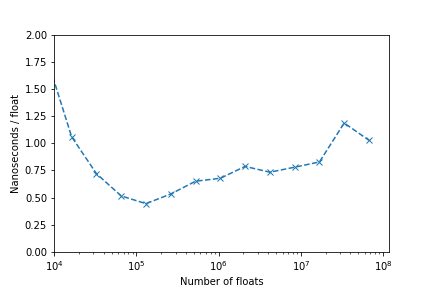
\includegraphics[width=6cm]{nanoseconds per float.png}     
 \end{center}

\begin{itemize}
    \item Laptop Frequency $\sim$ 2 GHz
    \item 1 Flop / cycle --- 0.5 ns / float
\end{itemize}

\end{frame}

\begin{frame}[fragile]
\frametitle{Memory bus}

Simple architecture model
 \begin{center}
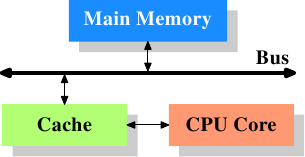
\includegraphics[width=5cm]{cpumemory.1.png}
\end{center}

\begin{itemize}
    \item Laptop Frequency: $\sim$ 2 GHz
    \item 1 Flop / cycle --- 0.5 ns / float
    \item DDR4 Bandwidth: $\sim$ 12 GByte/sec -- 0.66 ns / float
    \item Conclusion: Memory bandwidth is not a bottleneck single core of my laptop.
    \item In general, the performance can be memory-bound. 
\end{itemize}

\end{frame}

\begin{frame}[fragile]
\frametitle{The roofline model}

Arithmetic intensity: Number of Flop / Byte
 \begin{center}
\includesvg[width=7cm]{roofline.svg}
\end{center}

ToDo:
\begin{itemize}
    \item Check your peak compute performance.
    \item Check you memory bandwidth.
    \item Determine the minimum arithmetic intensity.
    \item Exercise: Optimize your memory access patterns! 
\end{itemize}

\end{frame}

\section{Performance of Deep Learning}


\frame{
\frametitle{Convolutional Neural Network}
Single convolution 128x128x16, 16 channels, float32
\begin{itemize}
    \item Input and output size: 1 MB , Weight size 2.25 kB (cached). 
    \item Total float ops: 72 MFlop. 
    \item Arithmetic intensity: $n_\text{out} \cdot k_x \cdot k_y / 4 $ =  36
    
    \item Peak Compute (A100): 21 TFlop/sec (FP32)
    \item GPU Memory Bandwidth (A100): 1.6 TByte / sec
    \item Minimum arithmetic intensity 13 (FP32)
    \item Peak Compute (A100): 151 TFlop/sec (TP32)
    \item Minimum arithmetic intensity 94 (TP32)
    

\end{itemize}
}

 
\frame{
\frametitle{The bottlenecks in DL}
\begin{tikzpicture}



%\node (start) [startstop] {Start};
\tikzstyle{startstop} = [rectangle, rounded corners, minimum width=0.5cm, minimum height=0.5cm,text centered, draw=black, fill=white]
\tikzstyle{io} = [trapezium, trapezium left angle=70, trapezium right angle=110, minimum width=3cm, minimum height=1cm, text centered, draw=black, fill=blue!30]
\tikzstyle{process} = [rectangle, minimum width=3cm, minimum height=1cm, text centered, draw=black, fill=orange!30]
\tikzstyle{decision} = [diamond, minimum width=3cm, minimum height=1cm, text centered, draw=black, fill=green!30]

\node (disk) [startstop] {
\includegraphics[height=12mm]{hd01.png} }; 
\node (memory) [startstop, right of=disk, xshift=2cm] {
\includegraphics[height=10mm]{ram.png}};
\node (gpumem) [startstop, right of=memory, xshift=2cm] {
\includegraphics[height=12mm]{gpu_card.png}};
\node (gpuproc) [startstop, right of=gpumem, xshift=2cm] {
\includegraphics[height=12mm]{gpu_proc.png}};

%\draw [->] (disk) --    node[anchor=north]{\rotatebox{-45}{File System}} (memory);
\draw [->] (disk) --    node[rotate=-45, anchor=north west,align=left]{File System} (memory);
\draw [->] (memory) -- node[rotate=-45, anchor=north west,align=left]{PCI Bus}  (gpumem);
\draw [->] (gpumem) -- node[rotate=-45, anchor=north west,align=left]{GPU Memory\\Bus } (gpuproc);
%\Strichmaxerl
\end{tikzpicture}

\begin{itemize}
    \item File System Bandwidth: 10 GByte /sec (its complicated)
    \item PCIe 4.0x16 Bandwidth: 32 GByte / sec
    \item GPU-GPU Bandwidth (NVLinkv3): 600 GByte / sec
    
    \item Peak Compute (A100): 21 TFlop/sec (FP32)
    \item GPU Memory Bandwidth (A100): 1.6 TByte / sec
\end{itemize}

}

\frame{
\frametitle{Case Analysis: ResNet50 Training on Imagenet}
\begin{itemize}
    \item Dataset size: 1.2 M Images, Training Resolution: 224x224x3
    \item Original Data: JPGs of different sizes, total 140 GB
    \item Uncompressed, resized to 224x224x3 data size: 180 GB
    \item PCIe limit 200k Images / sec.
    \item ResNet50 gradient computation: $\sim$ 20 GFlop.
    \item Compute Limit per GPU: (FP32) 1k Images / sec (TF32) 7k Images /sec
    \item Total weight size: 100 MB (float32)
    \item Dominating Operations: 3x3 Conv2D on 128x128x64, 64x64x128, 32x32x256, 16x16x512, Intensities: 144, 288, 576,1156
    
    %\href{test}{https://www.eenewseurope.com/news/resnet-50-misleading-machine-learning-inference-benchmark-megapixel-images/page/0/4}
\begin{center}
    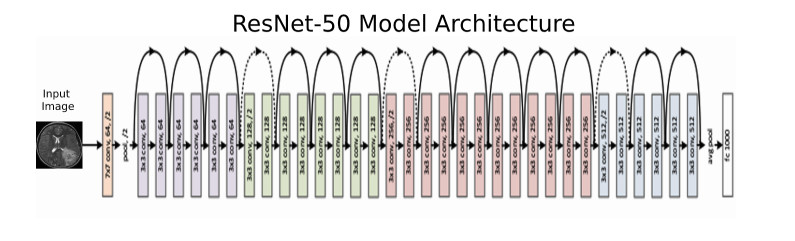
\includegraphics[width=0.9\textwidth]{resnet50.jpg}
\end{center}
\end{itemize}
}

\section{Building IO Pipelines}

\begin{frame}[fragile]
\frametitle{Serial Execution}
\begin{lstlisting}
def load_data():
    return np.random.normal(0,1, (224,224,3)),

# Define Model
inp=tf.compat.v1.placeholder(shape=(1,224,224,3),dtype=tf.float32 )
output = tf.keras.layers.Conv2D(16, kernel_size=(3,3), use_bias=False)(inp) 
# Prepare Session
sess=tf.compat.v1.Session()
sess.run(tf.compat.v1.initialize_all_variables())
# Run Model
data=load_data()
sess.run(output, feed_dict={inp: data })
\end{lstlisting}

\begin{center}
\timeserial    
\end{center}

    
\end{frame}


\begin{frame}{Prefetch: Asynchronous Execution}
\timebufferone
\vspace{1.0 cm}

\begin{itemize}
    \item Parallel execution of loading and  compute.
    \item Buffered: Load operation fills a buffer, compute consumes it.
    \item The buffer must be adjusted to the problem size.
    \item Example of latency hiding.
    \item Tensorflow dataset API: An easy way to do that.
\end{itemize}
    
\end{frame}



\frame{
\frametitle{Prefetch}

\timebuffer
\picprefetch[1.][6][12] {}

} % frame

\begin{frame}{The Dataset API}

    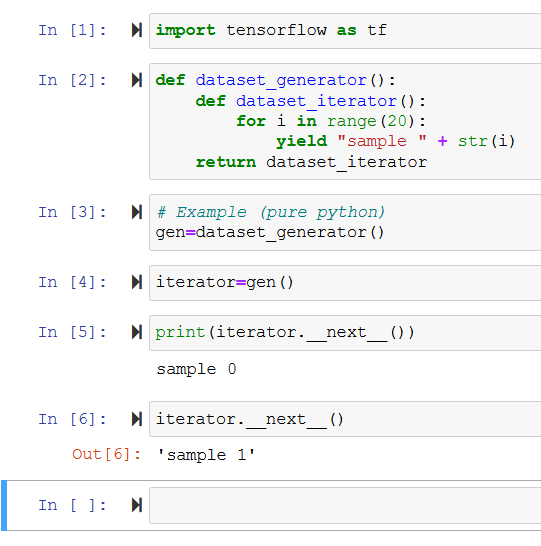
\includegraphics[width=0.4\textwidth]{dataset_pure_python.PNG}
    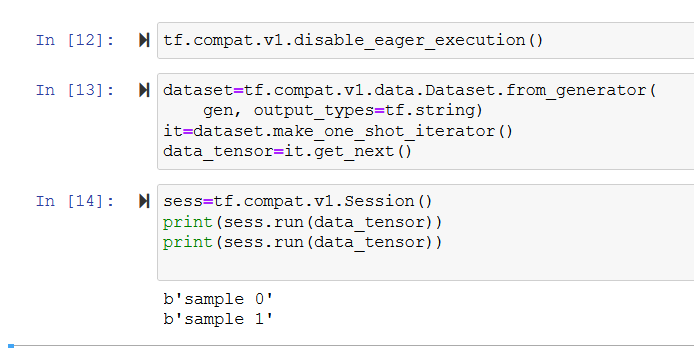
\includegraphics[width=0.59\textwidth]{dataset_tf1.PNG}
\end{frame}

\begin{frame}[fragile]{The Dataset API: TF2}

\begin{columns}
\begin{column}{0.5\textwidth}

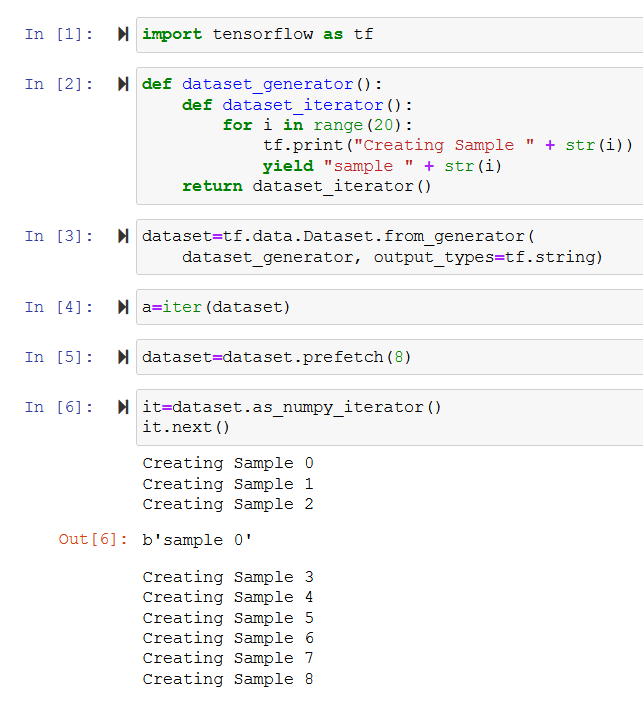
\includegraphics[height=0.8\textheight]{dataset_tf2.PNG}


\end{column}
\begin{column}{0.5\textwidth}  %%<--- here
    \begin{itemize}
        \item Eager execution: The compute graph is constructed on the fly.
        \item \texttt{from\_generator} receives a generator function, a callable that creates an iterator. So Keras can restart the iterator after each epoch.
        \item \texttt{Dataset}s can be transformed with a functional API
        \item \texttt{prefetch(<num>)} creates and fills a buffer.
    \end{itemize}
    
\end{column}
\end{columns}


    
\end{frame}

\begin{frame}{Shard}
    \picdatasetshard
    \begin{itemize}
        \item Using \texttt{shard(i,n)} will first skip the first $i$ entries in the dataset.
        \item Then it will skip $n$ entries.
        \item Thus you will get only those samples with index $k$,
        where $k\, \text{mod}\, n = i$.
        \item Thus, a not can get its shard, even random access is not available.
    \end{itemize}
\end{frame}

\begin{frame}{Batch}
    \picdatasetbatch
    \begin{itemize}
        \item \texttt{batch(n)} will accumulate $n$ samples and return a batched tensor.
        \item It will only load the samples after the next item was pulled, so combine with prefetch!
        \item The inverse operation is \texttt{unbatch}.
    \end{itemize}
\end{frame}

\begin{frame}{Shuffle}
    \picdatasetshuffle
    \begin{itemize}
        \item \texttt{shuffle(n)} buffer $n$.
        \item In each iteration, it will return a sample randomly from the buffer.
        \item The buffer is only refilled when needed. Combine with prefetch!
        \item Note that it yields only a limited randomization.
    \end{itemize}
\end{frame}

\begin{frame}{Map}
    \timetransformparallel
    \begin{itemize}
        \item \texttt{map(fun, n\_parallel\_calls} will apply a python function on each element.
        \item The execution is can be parallelized.
        \item (Pure) python and parallelization can be troublesome. Beware of the cliffs of \texttt{multiprocessing}!
    \end{itemize}
\end{frame}


\begin{frame}{Good practices}
    \begin{itemize}
        \item Store your data with a \textbf{transparent order} on disk. Otherwise you cannot do sequential read and this may be expensive.
        \item Do \textbf{not} store data in \textbf{many small files}. 
        \item Your dataset fits into the node's main memory? Easy. \textbf{Read sequentially}.
        \item Your dataset \textbf{does not fit} into main memory?
        \begin{itemize}
            \item Make sure you can read you data seqentially in chunks.
            \item Many relatively large files? OK. 
            \item File format with defined storage order and support for sequential reading? Perfect.
            \item Store data pre-shuffled. Otherwise you are likely to get random-access to HD.
        \end{itemize}
        \item Perform pre-processing on the fly, preferably directly in native tf, if necessary with parallel \texttt{map}.
    \end{itemize}
\end{frame}


\begin{frame}{Network Analysis}
\begin{itemize}
    \item Infiniband Bandwidth: $\sim$ 25-50 Gigabyte/sec.
    \item Infiniband Latency: 150 $\mu$s
    \item Model size (ResNet50): 100 MB $=$ 5 ms per transfer.
    \item No of transfers: $\sim 2 \log_2 n_\text{nodes}$
    \item Horovod periodically checks for \emph{finished} parts of the gradient. It will then start transferring if a threshold is exceeded.
\end{itemize}
%\centered{
%hello
%}
\only<1>{\commserial}
\only<2>{\commhidden}



    
\end{frame}

\begin{frame}{Horovod Timeline}
    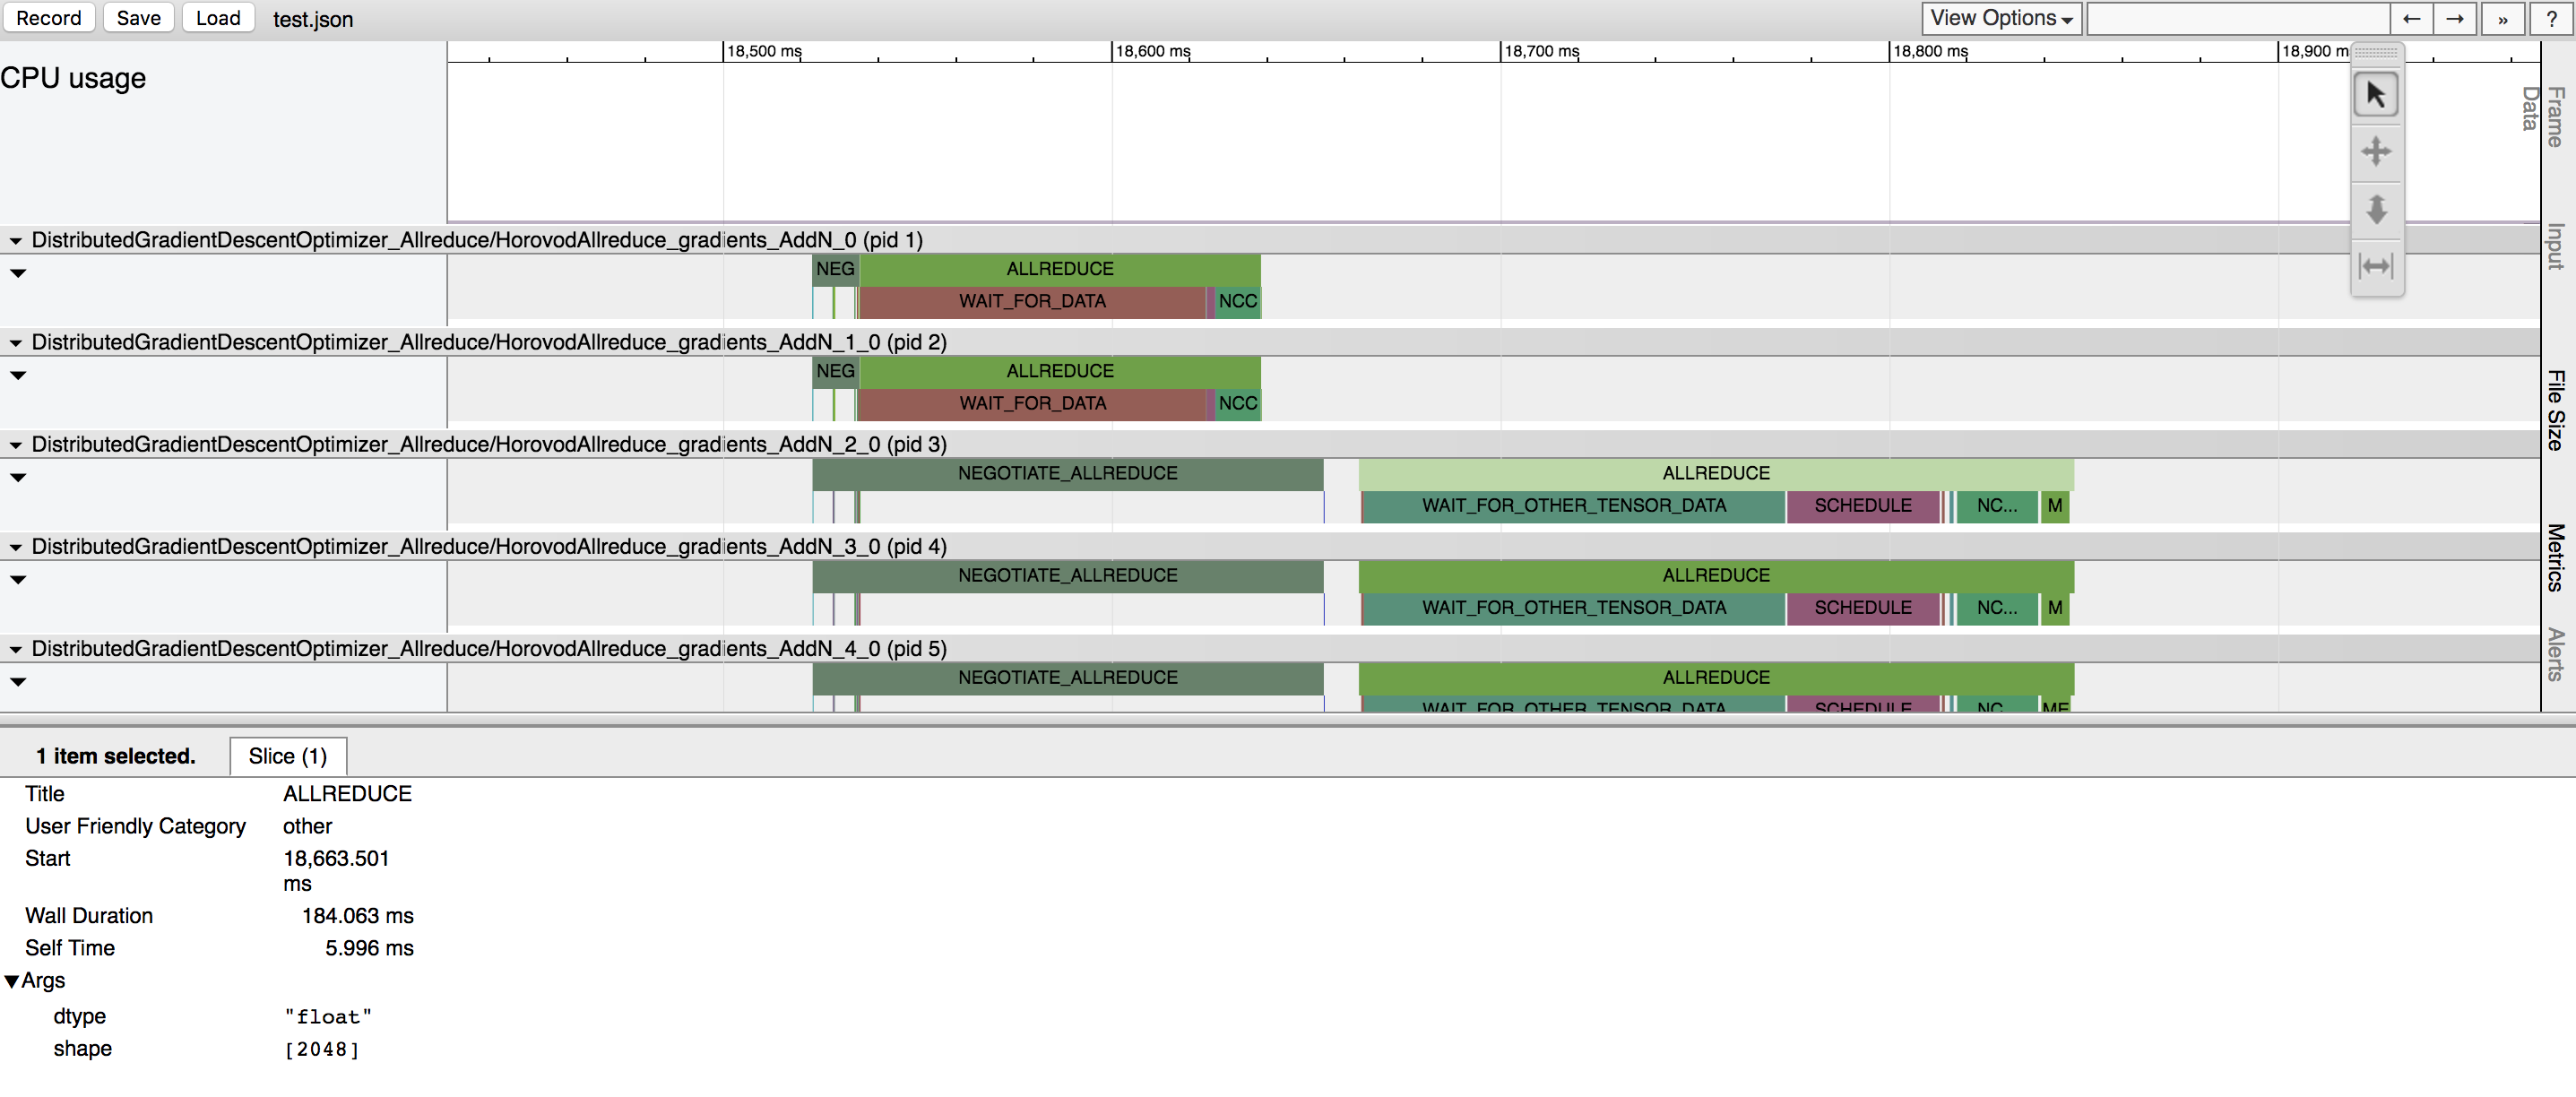
\includegraphics[width=0.8\textwidth]{horovod_timeline.png}
    \begin{itemize}
        \item Horovod Timeline: Get a timeline 
    of transfers
        \item Easy to use: \texttt{horovodrun -np 4 --timeline-filename /path/to/timeline.json python train.py}
        \item Open with chrome tracing.
    \end{itemize}
\end{frame}


\begin{frame}[fragile]{Tensorboard Profiler}

\includesvg[width=\textwidth]{vectorized_map}

Start with ssh tunnel in a single command on the login node:
\begin{lstlisting}
ssh -L 8889:localhost:53415 kesselheim1@juwels.fz-juelich.de "bash -c \"source /p/project/training2306/software_environment/activate.sh && tensorboard  --port 53415 --logdir /p/project/training2306/kesselheim1/ \" "
\end{lstlisting}
Navigate to http://localhost:8889

\textbf{Please change remote port from 53415 to you favourite random number above 1024}.

\end{frame}

\end{document}


\newlength{\iconheight}
\setlength{\iconheight}{12mm}
\newcommand{\hd}{
\includegraphics[height=\iconheight]{hd01.png}}
\newcommand{\gpugroup}{

\includegraphics[height=0.5\iconheight]{gpu_card.png}

\includegraphics[height=0.5\iconheight]{gpu_card.png} \\

\includegraphics[height=0.5\iconheight]{gpu_card.png}

\includegraphics[height=0.5\iconheight]{gpu_card.png}
}



\frame{
\frametitle{Bottlenecks on supercomputers}
Only a picture....\\
\begin{tikzpicture}

%\node (start) [startstop] {Start};
\tikzstyle{startstop} = [rectangle, rounded corners, minimum width=0.5cm, minimum height=0.5cm,text centered, draw=black, fill=white]
\tikzstyle{io} = [trapezium, trapezium left angle=70, trapezium right angle=110, minimum width=3cm, minimum height=1cm, text centered, draw=black, fill=blue!30]
\tikzstyle{process} = [rectangle, minimum width=3cm, minimum height=1cm, text centered, draw=black, fill=orange!30]
\tikzstyle{decision} = [diamond, minimum width=3cm, minimum height=1cm, text centered, draw=black, fill=green!30]

\node (disk) [startstop, align=left] {\hd \hd \\ \hd \hd \\ \hd \hd \\ \hd \hd };
\node (memory2) [startstop, right of=disk, xshift=2cm, align=left] {
\includegraphics[height=10mm]{ram.png}};
\node (memory1) [startstop, above of=memory2, yshift=+0.8cm, align=left] {
\includegraphics[height=10mm]{ram.png}};
\node (memory3) [startstop, below of=memory2, yshift=-0.8cm, align=left] {
\includegraphics[height=10mm]{ram.png}};

\node (gpumem2) [startstop, right of=memory2, xshift=2cm, align=left] {\gpugroup };
\node (gpumem1) [startstop, above of=gpumem2, yshift=+0.8cm, align=left] {\gpugroup };
\node (gpumem3) [startstop, below of=gpumem2, yshift=-0.8cm, align=left] {\gpugroup };

\node (gpuproc2) [startstop, right of=gpumem2, xshift=2cm] {
\includegraphics[height=12mm]{gpu_proc.png}};
\node (gpuproc1) [startstop, above of=gpuproc2, yshift=+0.8cm] {
\includegraphics[height=12mm]{gpu_proc.png}};
\node (gpuproc3) [startstop, below of=gpuproc2, yshift=-0.8cm] {
\includegraphics[height=12mm]{gpu_proc.png}};

%\draw [->] (disk) --    node[anchor=north]{\rotatebox{-45}{File System}} (memory);
\draw [->] (disk) --   (memory1);
\draw [->] (disk) --   (memory2);
\draw [->] (disk) --   (memory3);
\draw [->] (memory1) --  (gpumem1);
\draw [->] (memory2) --  (gpumem2);
\draw [->] (memory3) --  (gpumem3);
\draw [->] (gpumem1) -- node[anchor=south] {4x} (gpuproc1);
\draw [->] (gpumem2) -- node[anchor=south] {4x} (gpuproc2);
\draw [->] (gpumem3) -- node[anchor=south] {4x} (gpuproc3);
\end{tikzpicture}



}

\tikzset{
    *-/.style={
        to path={
            (perpendicular cs: horizontal line through={(\tikztostart)},
                                 vertical line through={(\tikztotarget)})
            % is the same as (\tikztostart -| \tikztotarget)
            % but just to be safe: http://tex.stackexchange.com/a/29781/16595
            -- (\tikztotarget) \tikztonodes
        }
    }
}




\end{document}
